\chapter{Analisis}
\label{chap:analisis}

\section{Analisis Perangkat Lunak Sejenis}
\label{sec:analisis pl}

Salah satu \textit{website} yang dapat memberikan rekomendasi program studi adalah \url{https://rencanamu.id}. \textit{Website} tersebut dikembangkan menggunakan riset ilmiah, Rencanamu mengukur 7 dimensi profil siswa sebagai landasan dalam rekomendasi, perencanaan kuliah dan karier yang terintegrasi, berkesinambungan dan menyeluruh. Gambar \ref{gambar31} menunjukkan 7 dimensi profil siswa. % https://rencanamu.id/about-us

\begin{figure}[H]
    \centering
    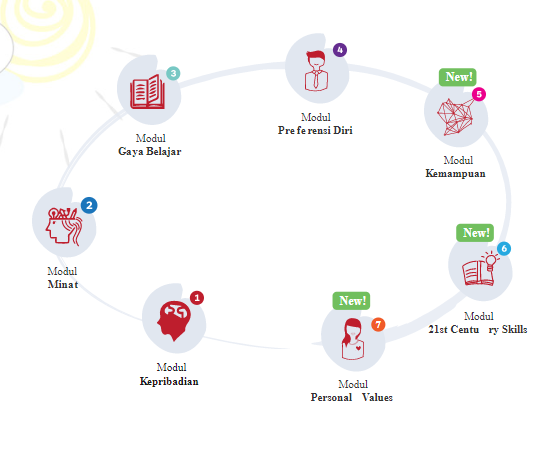
\includegraphics[width = 10cm, height = 10cm]{doc/DokumenSkripsi/Gambar/gambar31.PNG}
    \caption{7 Dimensi Profil Siswa}
    \label{gambar31}
\end{figure}

Pada \textit{website} ini, telah dilakukan beberapa analisis dan hasilnya sebagai berikut :

\begin{enumerate}
    \item \textit{Website} \url{https://rencanamu.id} adalah sebuah \textit{platform} persiapan kuliah dan karier \textit{online} berbasis data didukung oleh teknologi \textit{People Science} untuk membantu siswa dalam merancang dan mempersiapkan masa depan mereka. 
    
    \item Perlu melakukan registrasi atau \textit{login} kedalam \textit{website}.
    
    \item Gambar \ref{gambar32} merupakan tampilan awal setelah registrasi atau \textit{login}.
    
    \begin{figure}[H]
        \centering
        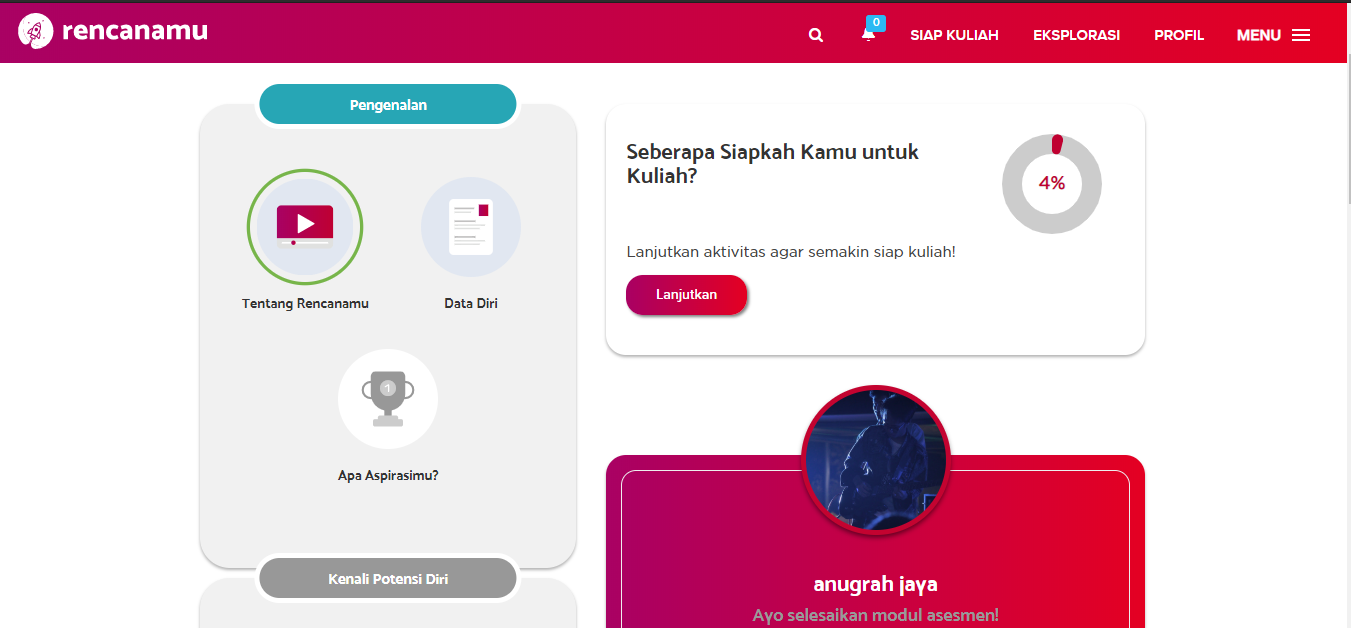
\includegraphics[width = 8cm, height = 5 cm]{doc/DokumenSkripsi/Gambar/gambar32.PNG}
        \caption{Tampilan setelah registrasi atau \textit{login}}
        \label{gambar32}
    \end{figure}
    
    \item Gambar \ref{gambar33}, Gambar \ref{gambar34}, dan Gambar \ref{gambar35} adalah beberapa modul yang harus dikerjakan.
    
    \begin{figure}[H]
        \centering
        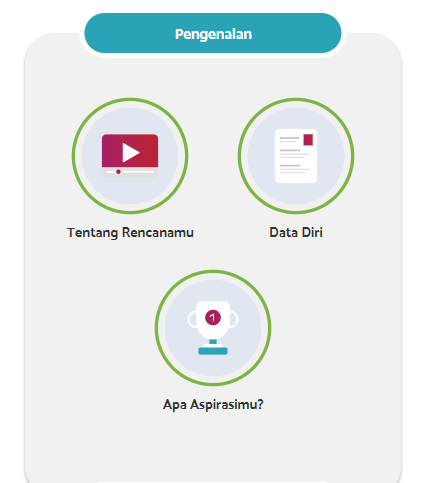
\includegraphics[width = 6cm, height = 7cm ]{doc/DokumenSkripsi/Gambar/gambar33.PNG}
        \caption{Caption}
        \label{gambar33}
    \end{figure}
    
    \begin{figure}[H]
        \centering
        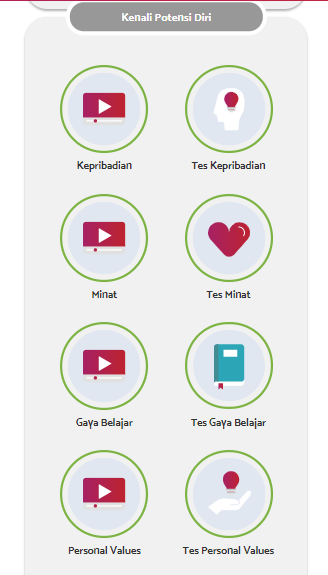
\includegraphics[width = 6cm, height = 9cm ]{doc/DokumenSkripsi/Gambar/gambar34.PNG}
        \caption{Caption}
        \label{gambar34}
    \end{figure}
    
    \begin{figure}[H]
        \centering
        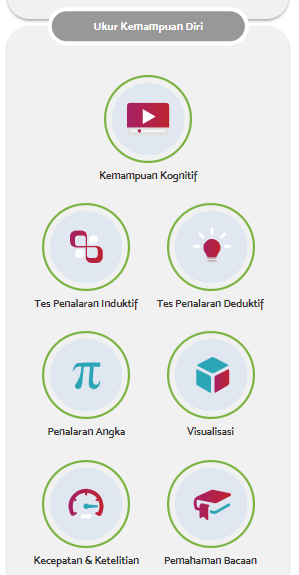
\includegraphics[width = 6cm, height = 8cm ]{doc/DokumenSkripsi/Gambar/gambar35.PNG}
        \caption{Caption}
        \label{gambar35}
    \end{figure}
    
    \item Gambar \ref{gambar36} adalah contoh hasil rekomendasikan yang diberikan sistem berdasarkan modul yang sudah dikerjakan.
    
    \begin{figure}[H]
        \centering
        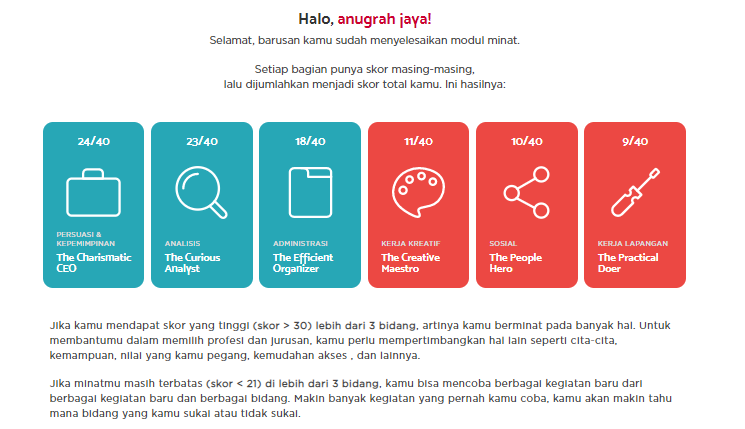
\includegraphics[width = 7cm, height = 8cm ]{doc/DokumenSkripsi/Gambar/gambar36.PNG}
        \caption{Hasil Rekomendasi}
        \label{gambar36}
    \end{figure}
    
\end{enumerate}

\textit{Website} \url{https://rencanamu.id} memiliki kesamaan dengan \textit{website} yang dibangun yaitu memberikan rekomendasi program studi untuk anak SMA. Perbedaannya pada \textit{website} \url{https://rencanamu.id} tidak menampilkan prediksi IPK dan harus mengisi beberapa modul untuk mendapatkan rekomendasi program studi. 

\section{Pemilihan Algoritma Sistem Rekomendasi}
Berdasarkan teori \ref{teknik rekomendasi} yang menjelaskan mengenai teknik-teknik yang dapat digunakan untuk membangun sistem rekomendasi, teknik \textit{collaborative filtering} adalah teknik yang dapat digunakan untuk memberikan rekomendasi berupa program studi kepada calon mahasiswa berdasarkan kesamaan dengan pengguna lain. Berikut merupakan beberapa hal mengapa memilih teknik \textit{collaborative filtering} :

\begin{enumerate}
    \item \textit{Collaborative filtering} menghasilkan rekomendasi item yang spesifik untuk pengguna berdasarkan peringkat tanpa memerlukan informasi tambahan mengenai item ataupun pengguna.
    
    \item 
\end{enumerate}

Teknik \textit{collaborative filtering} memiliki beberapa kekurangan diantaranya : 

\begin{enumerate}
    \item Rekomendasi yang diberikan mengambil data yang cukup banyak dari basis data sehingga membutuhkan memori yang besar.
    
    \item Tidak bisa memberikan rekomendasi untuk item yang tidak pernah diberikan \textit{rating} oleh pengguna.
    
    \item Pengguna harus memberikan \textit{rating} untuk beberapa item agar bisa diberikan rekomendasi.
\end{enumerate}

Pada \textit{website} yang dibangun, akan memberikan rekomendasi berdasarkan nilai raport beberapa mata pelajaran siswa pada kelas 10 dan 11. Rekomendasi program studi berdasarkan asal jurusan saat SMA, misalnya siswa IPA akan diberikan rekomendasi program studi IPA.

\section{Analisis Bobot Nilai Berdasarkan Aktivitas Pengguna}

\section{Contoh Perhitungan Pearson Correlation}

\subsection{\textit{Framework} Laravel}

\subsection{\textit{Framework} Bootstrap}

\section{Analisis Kebutuhan Sistem}

\subsection{Rancangan Basis Data}
% erd, table, skema relasi

% perlu atau engga ? kata bu mar ga terlalu perlu
\subsection{Diagram \textit{Use-Case}}

